\documentclass{beamer}
\usetheme{Boadilla}
\usepackage{ulem}
\usepackage{xspace}
\usepackage{xcolor}
\usepackage{centernot}

% Formatting/color
\definecolor{ReedRed}{RGB}{ 167, 14, 22} 
\definecolor{ReedGrey}{RGB}{ 191, 175, 159}
\definecolor{ReedRed2}{RGB}{ 94, 5, 1}

\setbeamercolor{palette primary}{bg=ReedRed,fg=white}
\setbeamercolor{palette secondary}{bg=ReedRed2, fg=white}
\setbeamercolor{palette tertiary}{bg=ReedRed,fg=white}
\setbeamercolor{palette quaternary}{bg=ReedRed,fg=white}
\setbeamercolor{structure}{fg=ReedRed} % itemize, enumerate, etc
\setbeamercolor{title}{fg=ReedRed} % itemize, enumerate, etc

\useinnertheme{circles} %replace shiny circles with normal ones

\newcommand{\sse}{\textit{SSE}\xspace}
\newcommand{\ssa}{\textit{SSA}\xspace}
\newcommand{\se}{\textit{SE}\xspace}
\newcommand{\sa}{\textit{SA}\xspace}
\newcommand{\lap}{\ensuremath{{\sf Lap}}\xspace}


\beamertemplatenavigationsymbolsempty

\title[Improved Private ANOVA]{Improved Differentially Private Analysis of Variance}
\author[Marika Swanberg]{\textcolor{blue}{Marika Swanberg} \and Ira Globus-Harris \and Iris Griffith \and \newline Anna Ritz \and  Andrew Bray \and Adam Groce}
\date{}

\begin{document}

\begin{frame}
\titlepage

\begin{figure}[!tbp]
  \centering
  \begin{minipage}[b]{0.45\textwidth}
    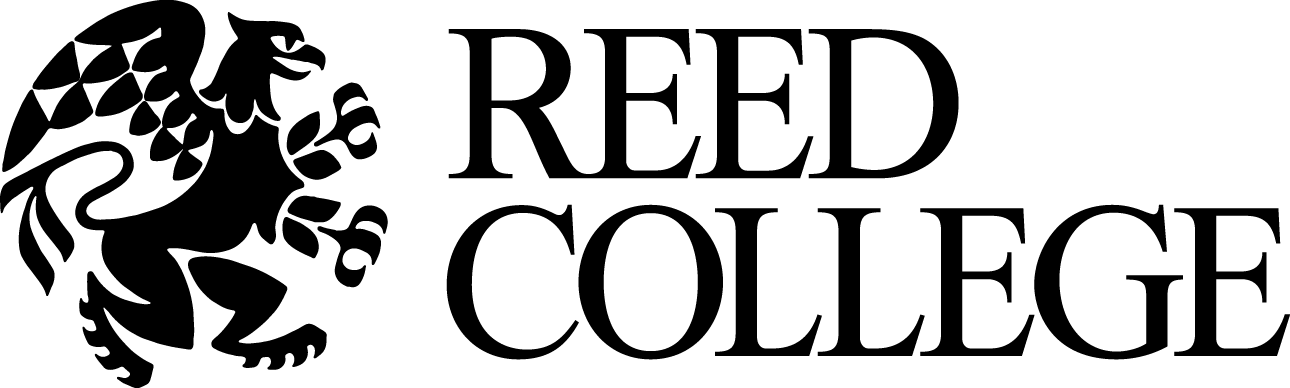
\includegraphics[width=\textwidth]{images/reed-logo}
  \end{minipage}
  \hfill
  \begin{minipage}[b]{0.45\textwidth}
    
\includegraphics[width=\textwidth]{images/BU-logo}
  \end{minipage}
\end{figure}

\end{frame}

%\begin{frame}{Outline}
%  \tableofcontents
%  % You might wish to add the option [pausesections]
%\end{frame}

% Section and subsections will appear in the presentation overview
% and table of contents.
\section{Differential Privacy}

\begin{frame}{Observed Data, $n=30$}
\pause
\begin{figure}
  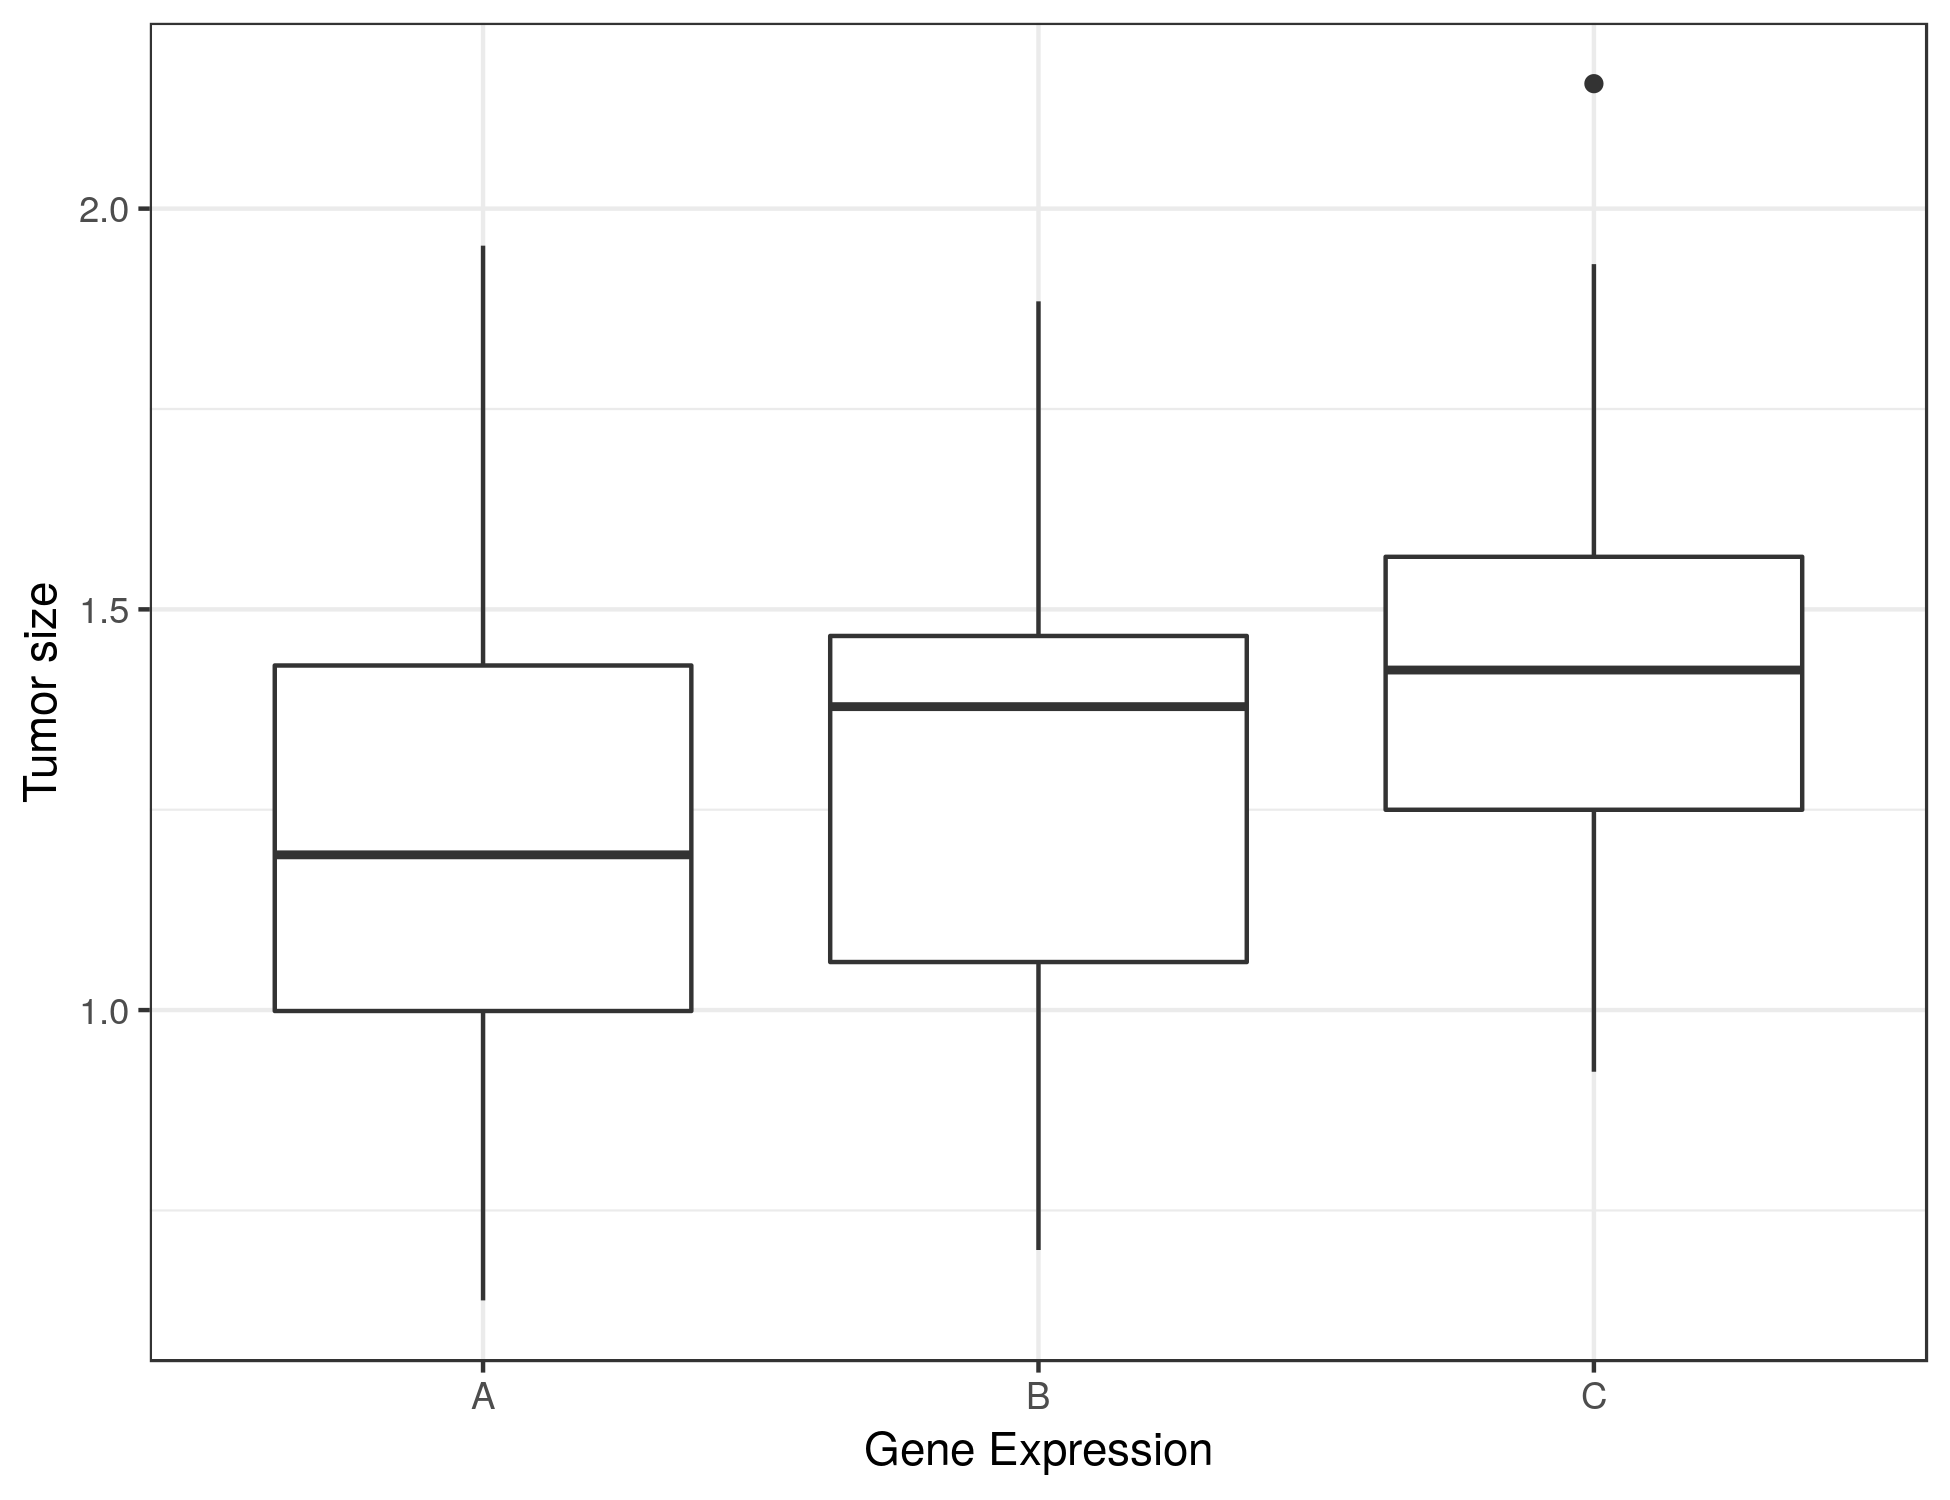
\includegraphics[scale=0.5]{simulation/observed-plot}
\end{figure}
\pause
Random variation or real dependency?
\end{frame}

\begin{frame}{Analysis of Variance Metric}
\pause
\begin{equation*}
 \frac{\text{Variation between groups}}{\text{In-group variation}} \pause 
\end{equation*}
\pause
The metric:
\begin{equation*}
\ssa(D) = \sum_{j=1}^{k} n_j (\bar{y}_j - \bar{y})^2
\end{equation*}

\begin{equation*}
\sse(D) = \sum_{i=1}^{n}  (y_{i}-\bar{y}_{c_i})^2
\end{equation*}
\begin{equation*}
F = \frac{\ssa/(k-1)}{\sse/(n-k)}
\end{equation*}
\end{frame}

\begin{frame}{Observed Data, $n=30$}
\begin{figure}
  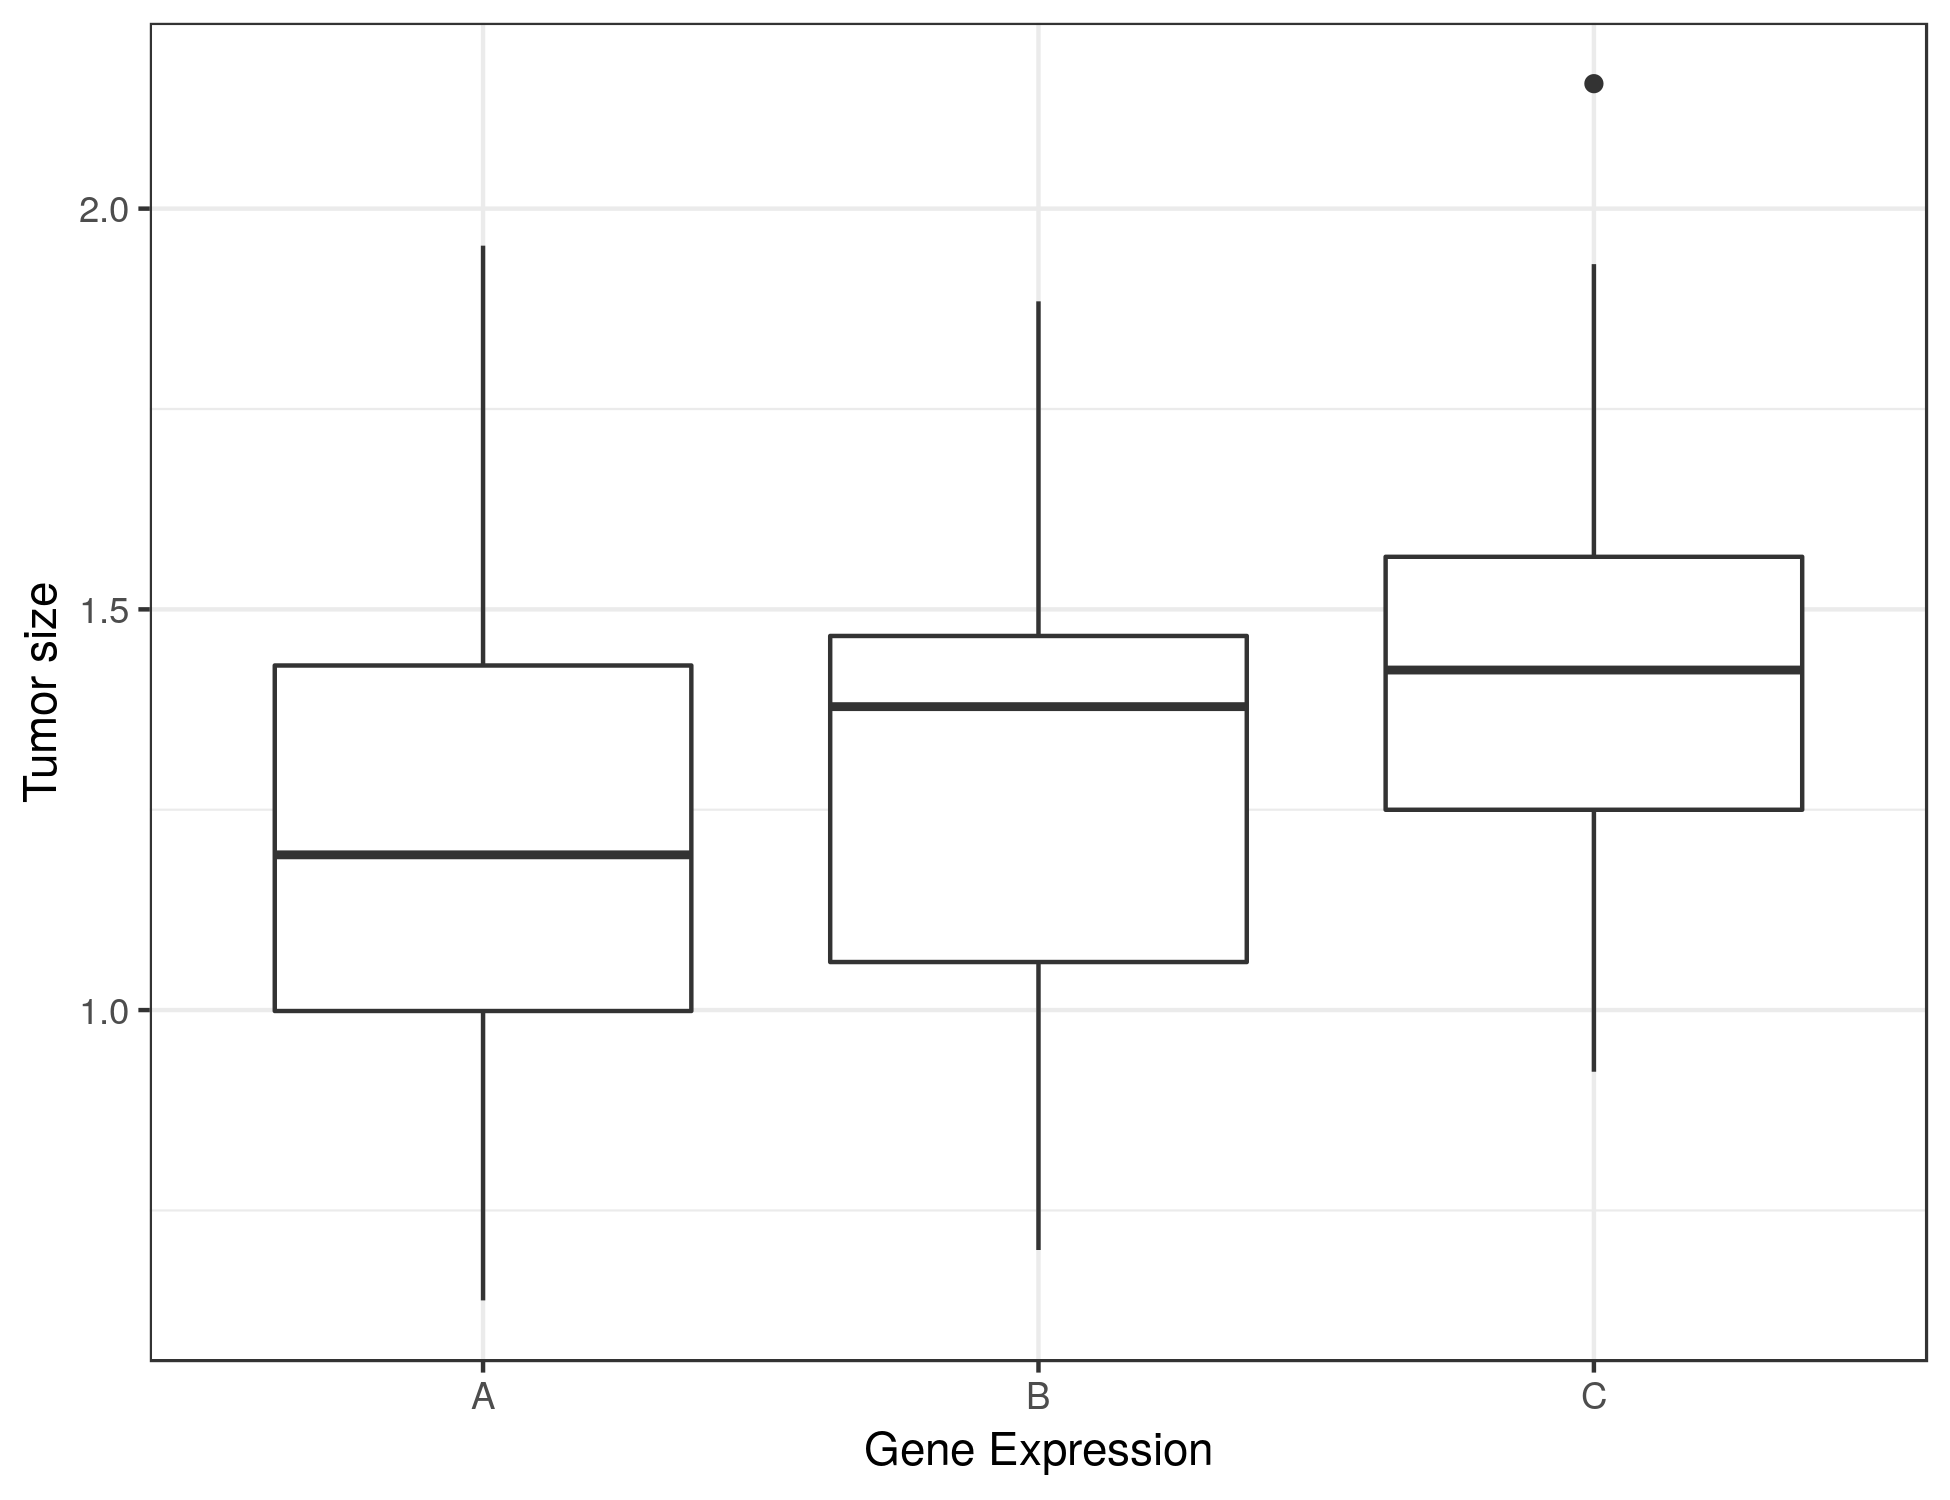
\includegraphics[scale=0.5]{simulation/observed-plot}
\end{figure}
\centering
$F = 4.988$
\end{frame}


\begin{frame}{Simulate Null Data}
\pause
\begin{figure}
  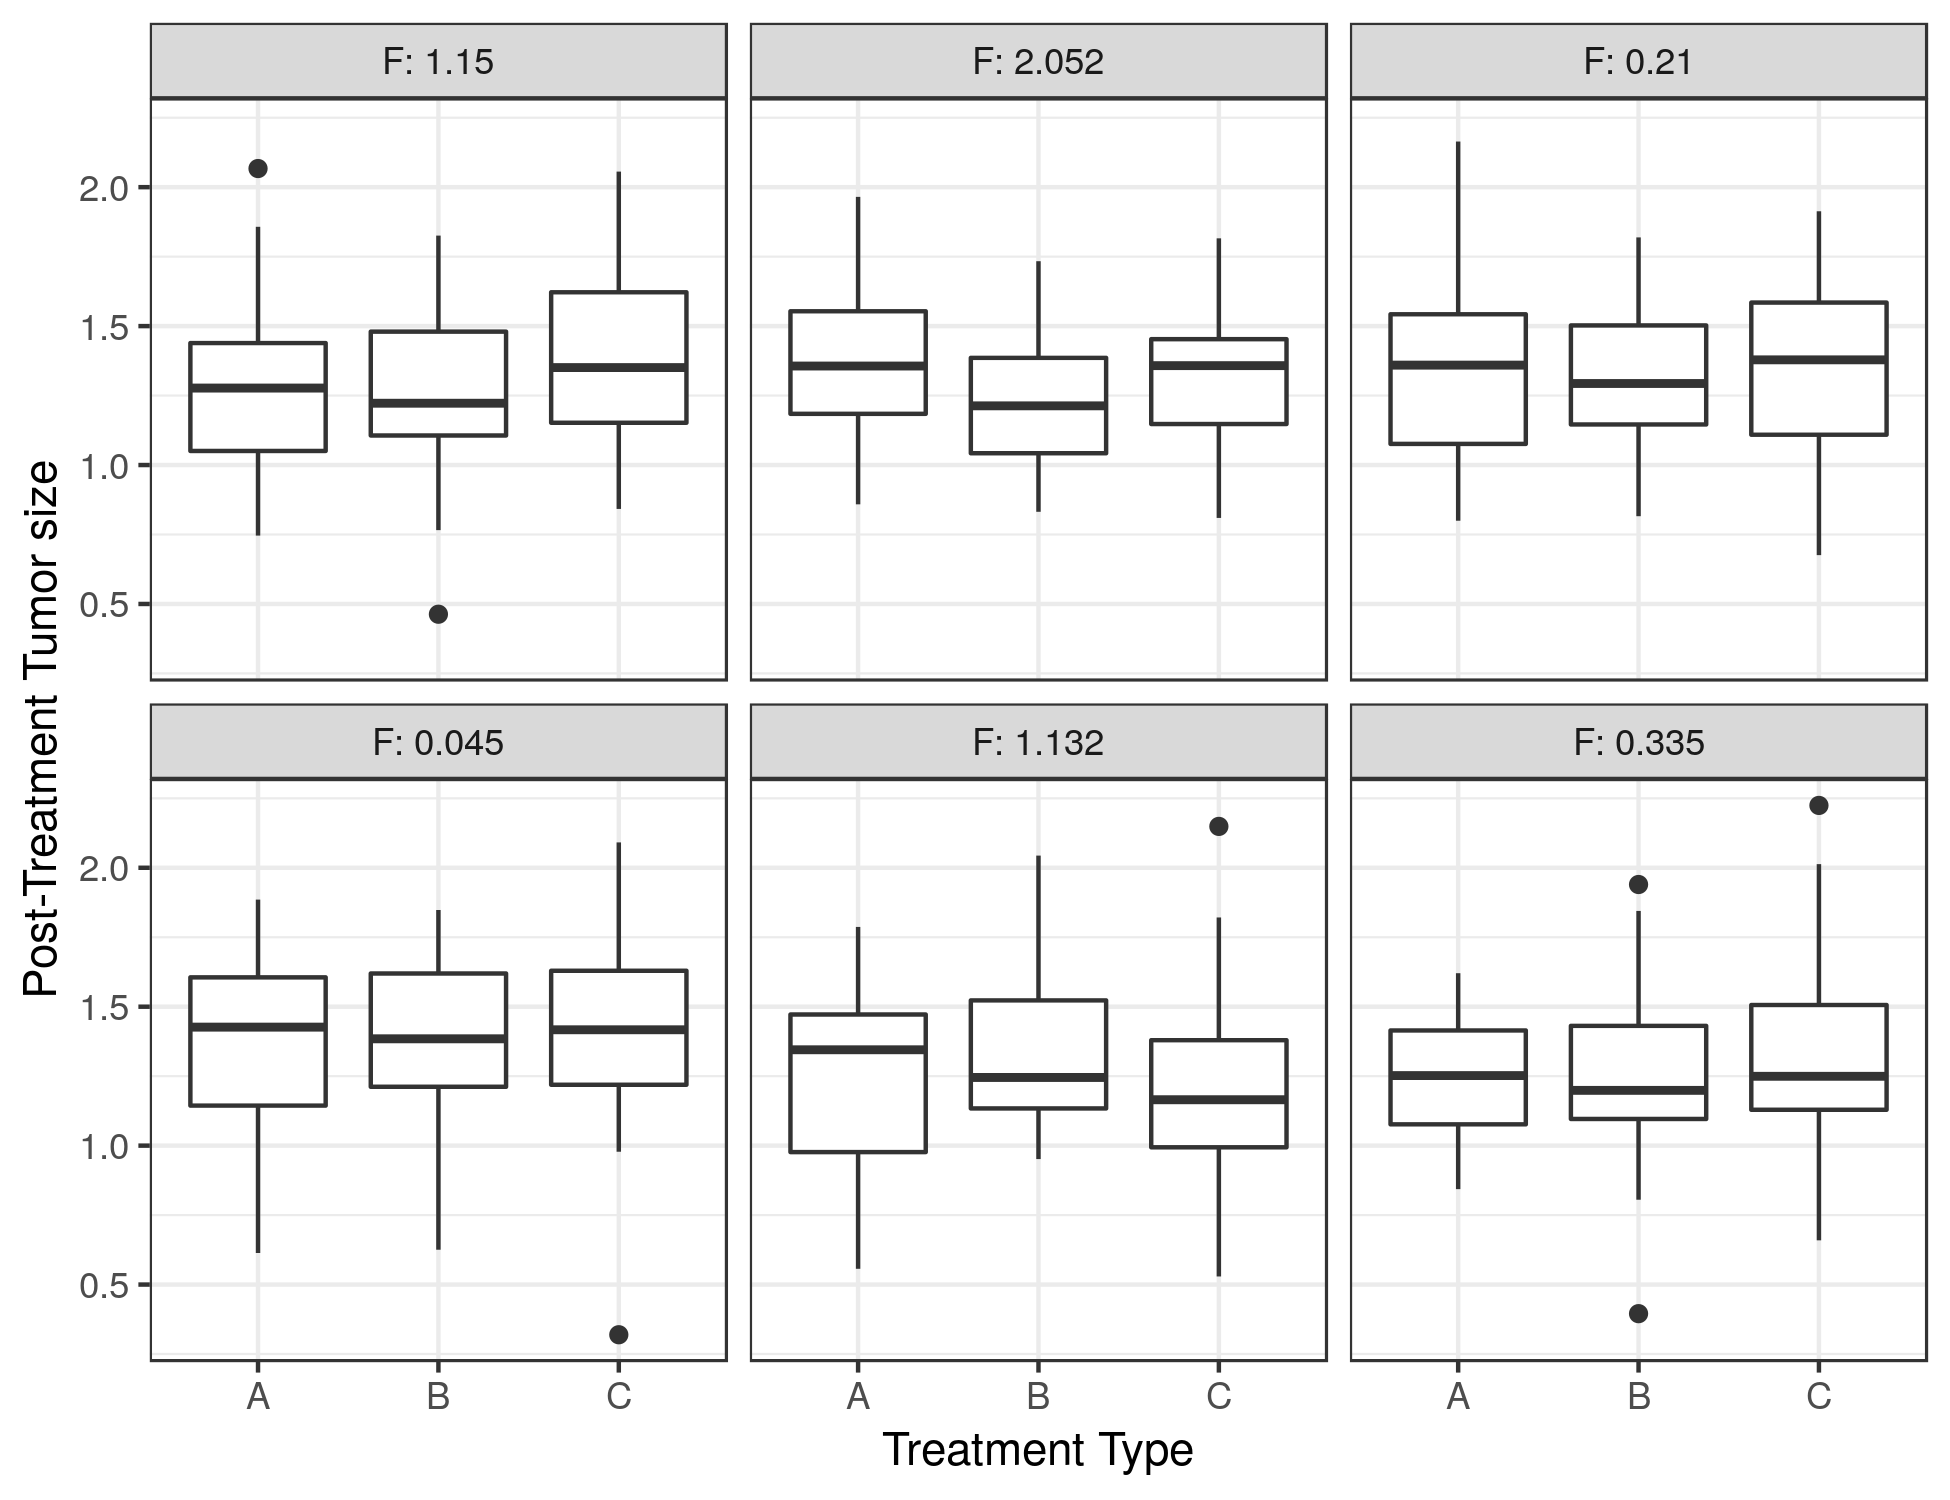
\includegraphics[scale=0.60]{simulation/null-plots}
\end{figure}
\end{frame}

\begin{frame}{}
\begin{figure}
  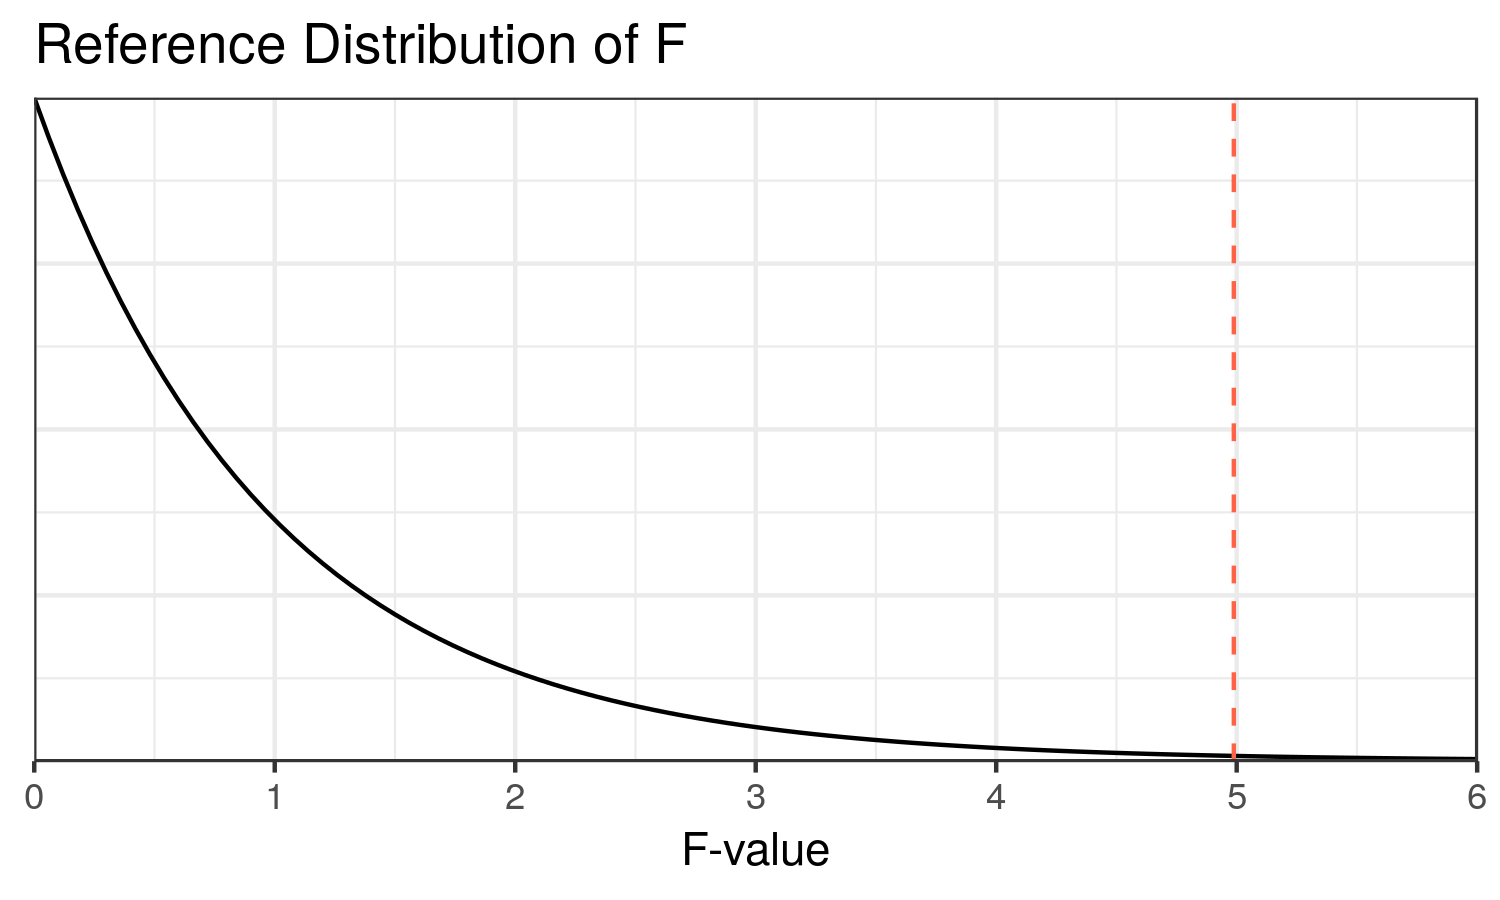
\includegraphics[scale=0.9]{simulation/null-dist}
\end{figure} 
\end{frame}

\begin{frame}{Why is $F$-test optimal?}
\pause
High probability of indicating dependence when variables \emph{are} dependent \ldots\pause  

\bigskip
\ldots even when dataset is small.

\pause
\begin{definition}[Power]
The \textbf{power} of a hypothesis test is the probability it rejects $H_0$.  It depends on the alternate distribution $H_A$ and $n$.
\end{definition}
\bigskip 

\pause
Goal of any test statistic is achieving high power$^*$.
\end{frame}

\begin{frame}{Observed Data, $n=30$}
\begin{figure}
  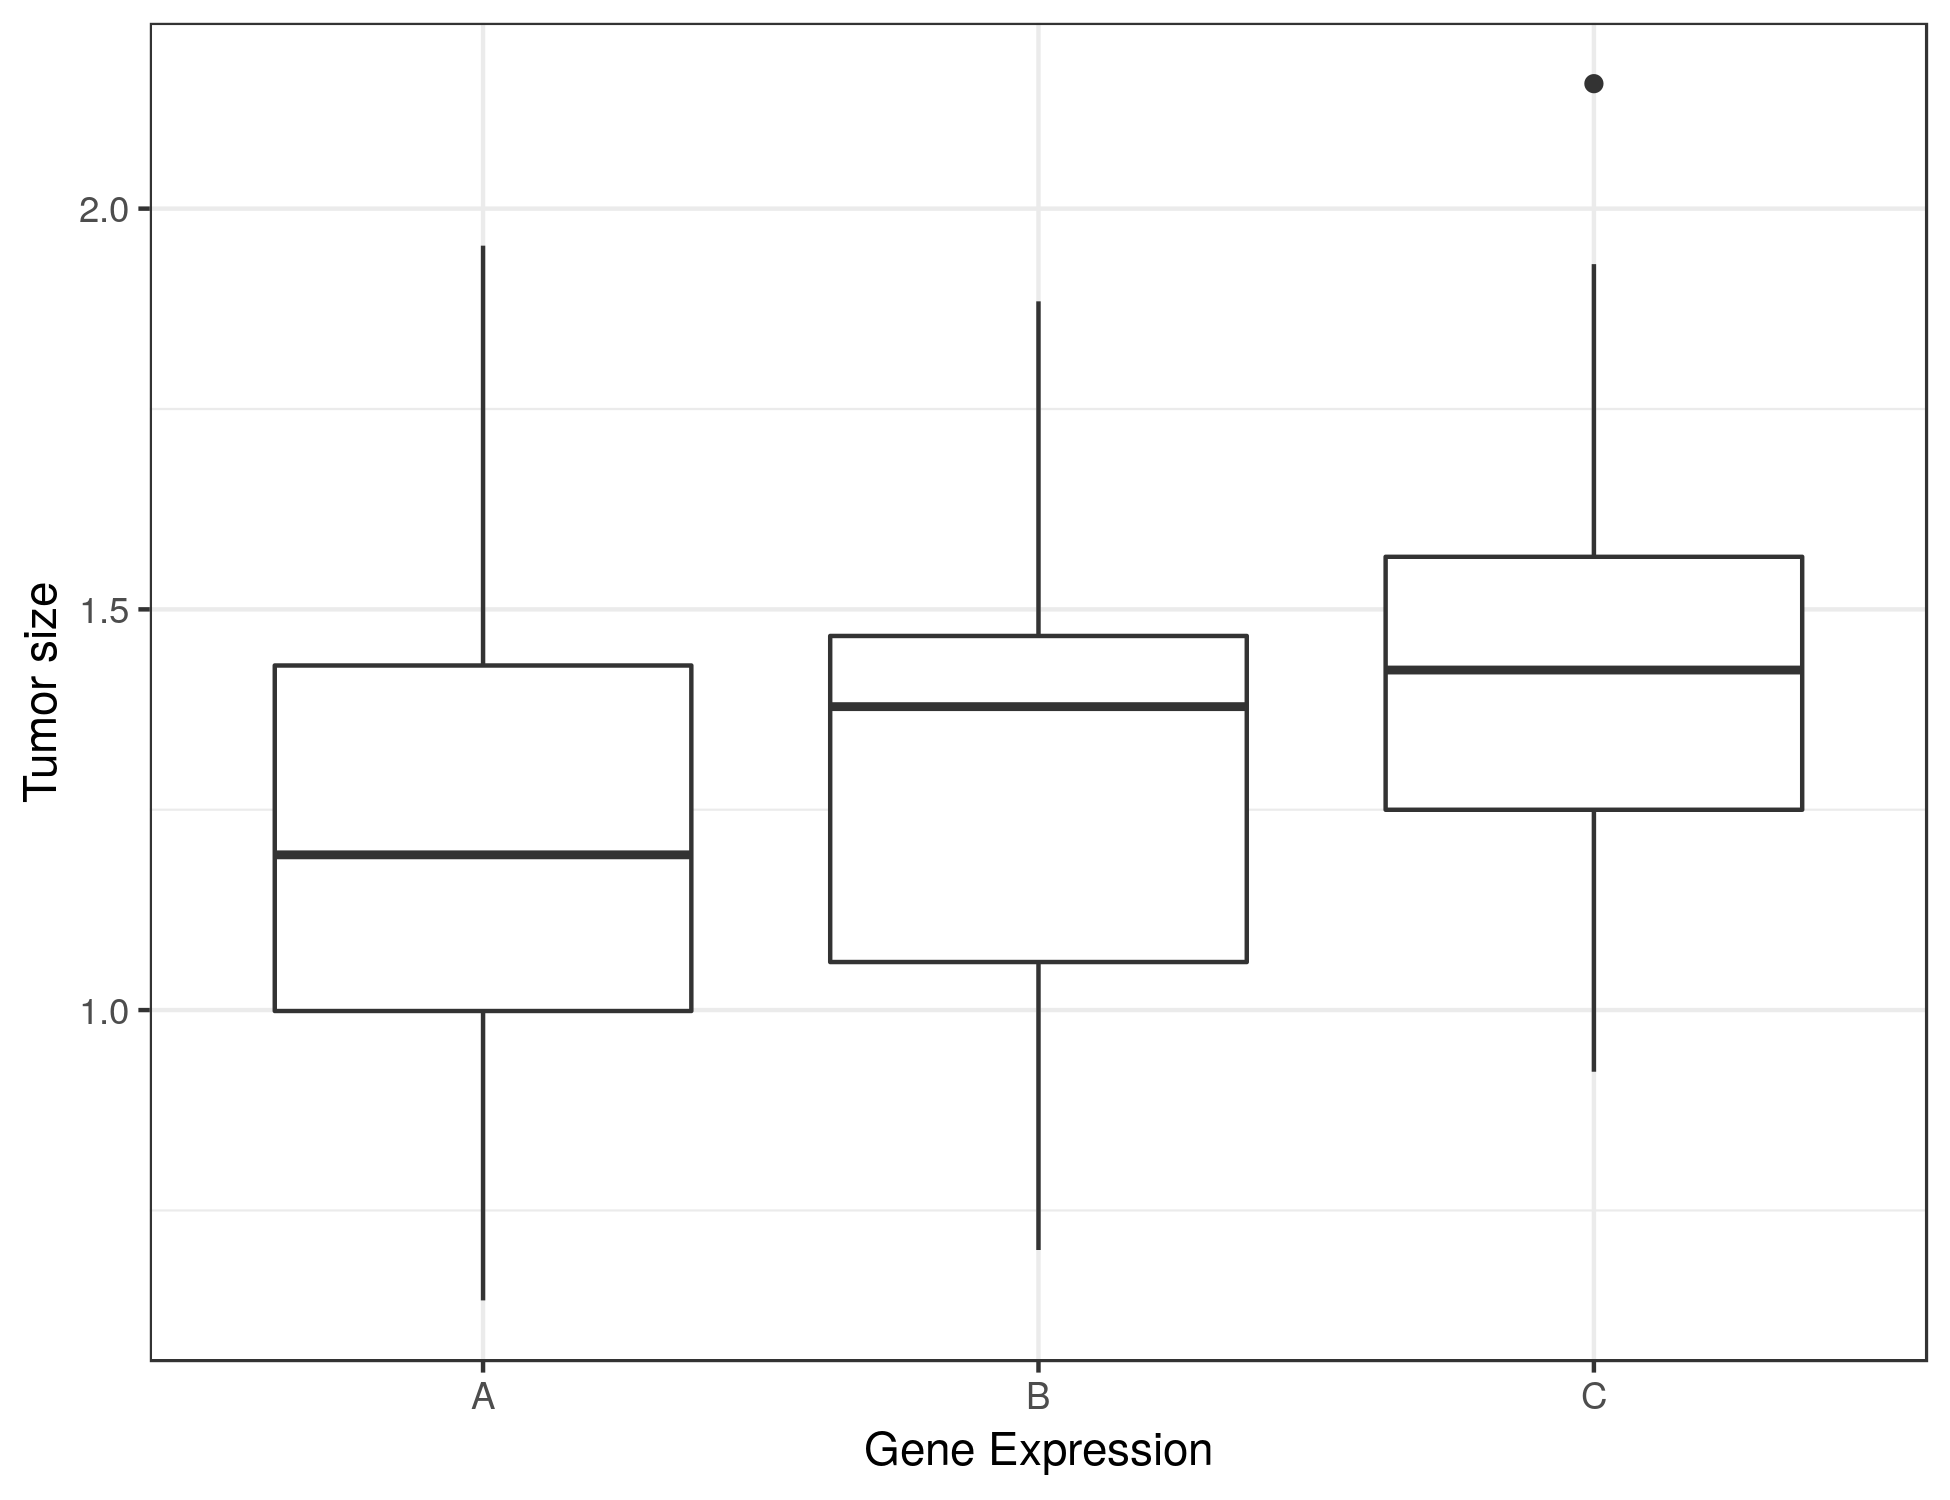
\includegraphics[scale=0.5]{simulation/observed-plot}
\end{figure}
What if we want to keep this data private?
\end{frame}

% SLIDE 3
\begin{frame}{Differential privacy [DMNS06]}
\pause
\begin{definition}
Two databases are \textbf{neighboring} if they differ only in the data of one individual.
\end{definition}
\pause
\begin{definition}
A query $f$ is \textbf{$\varepsilon$-differentially private} if for all neighboring databases $D, D'$ and all output sets $S$
\begin{equation*}
\Pr[f(D) \in S] \leq e^\varepsilon \Pr[f(D') \in S].
\end{equation*}
\end{definition}
\end{frame}

% SLIDE 4
\begin{frame}{Properties of differential privacy [DMNS06]}
\pause
\begin{theorem}[Post-processing]
If $f$ is $\varepsilon$-differentially private then for any (randomized) function $g$, then if $h(D) = g(f(D))$, $h$ is also $\varepsilon$-differentially private.
\end{theorem}
\pause
\begin{theorem}[Composition]
If $f$ is $\varepsilon_1$-differentially private and $g$ is $\varepsilon_2$-differentially private then if $h(D) = (g(D), f(D))$, $h$ is  $(\varepsilon_1+\varepsilon_2)$-differentially private.
\end{theorem}
\end{frame}

% SLIDE 5
\begin{frame}{Laplace mechanism [DMNS06]}
\pause
\begin{definition}[Sensitivity]
The sensitivity $\Delta f$ of a deterministic, real-valued function $f$ on databases is the maximum over all pairs of neighboring $D, D'$ of $| f(D) - f(D') |$.
\end{definition}

\pause
\begin{theorem}[Laplace Mechanism]
Given any deterministic, real-valued function $f$ on databases, define $\widehat{f}$ as
$$\widehat{f}(D) = f(D) + Y,$$
where $Y \leftarrow \lap(\Delta f/\varepsilon)$. The Laplace mechanism is $\varepsilon$-differentially private.
\end{theorem}
\end{frame}

% SLIDE 5
\begin{frame}{Related Works}
    Other work on private hypothesis testing:\pause
\begin{itemize}
\item Asymptotic analysis [WZ10, Smith11, CKMSU19] \pause
\item Chi-squared test (difference of discrete distributions) [VS09, FSU11, JS13, USF13, WLK15, GLRV16, RK17] \pause
\item Other tests: \pause
\begin{itemize}
\item Binomial data [AS18] (Proven optimal!) \pause
\item Difference of two means [OHK15, DNLI18] \pause
\item Linear regression [BRMC17, Sheffet17] \pause
\end{itemize}
\end{itemize}
Earlier work is often missing: \pause
\begin{itemize}
\item Accurate $p$-value computations \pause
\item Demonstrated validity of $p$-values \pause
\item Power analysis
\end{itemize}
\end{frame}

\begin{frame}{Private $F$-statistic [CBRG18]}
\pause
Assume data is on the $[0,1]$ interval. \pause
\begin{theorem}
\sse has sensitivity bounded by 7.
\end{theorem}
\begin{theorem}
\ssa has sensitivity bounded by $9 + 5/n$.
\end{theorem}
\pause
$$\widehat{\sse}(D) = \sse(D) + \lap\left(\frac{7}{\varepsilon/2}\right) $$

$$\widehat{\ssa}(D) = \ssa(D) + \lap\left(\frac{9+5/n}{\varepsilon/2}\right) $$ 
\end{frame}

% SLIDE 9
\begin{frame}{Private ANOVA [CBRG18]}
$$\widehat{F}(D) = \frac{\widehat{\ssa}(D)/(k-1)}{\widehat{\sse}(D)/(n-k)}$$
\bigskip

 \pause
 \centering
Problem: What is the reference distribution now? \pause
\begin{figure}
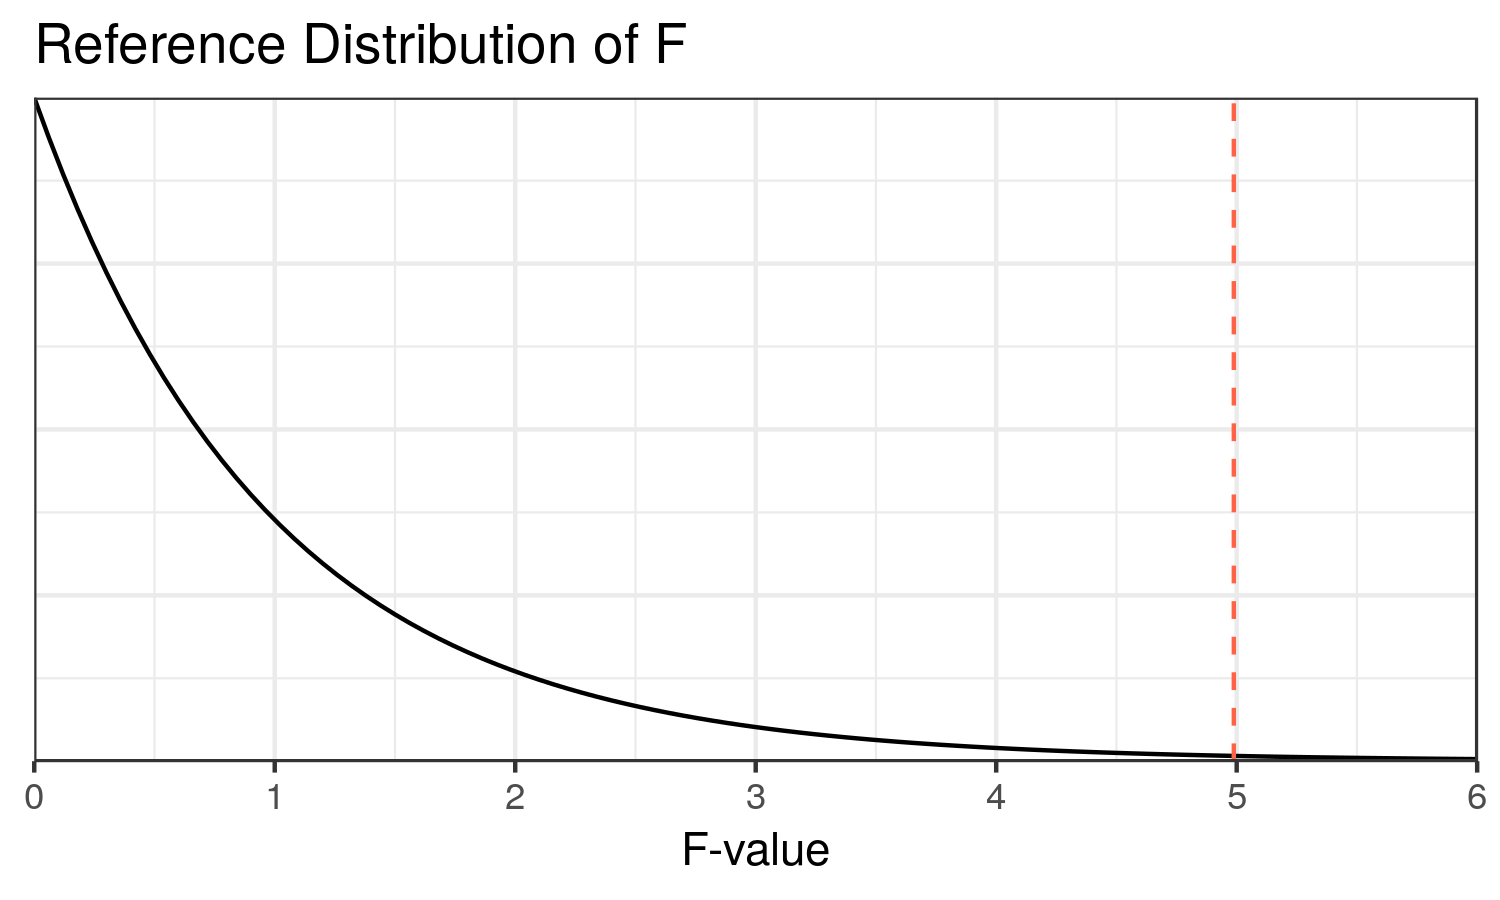
\includegraphics[scale=0.7]{simulation/null-dist}
\end{figure}
\end{frame}


\begin{frame}{Private ANOVA [CBRG18]}
\begin{figure}
  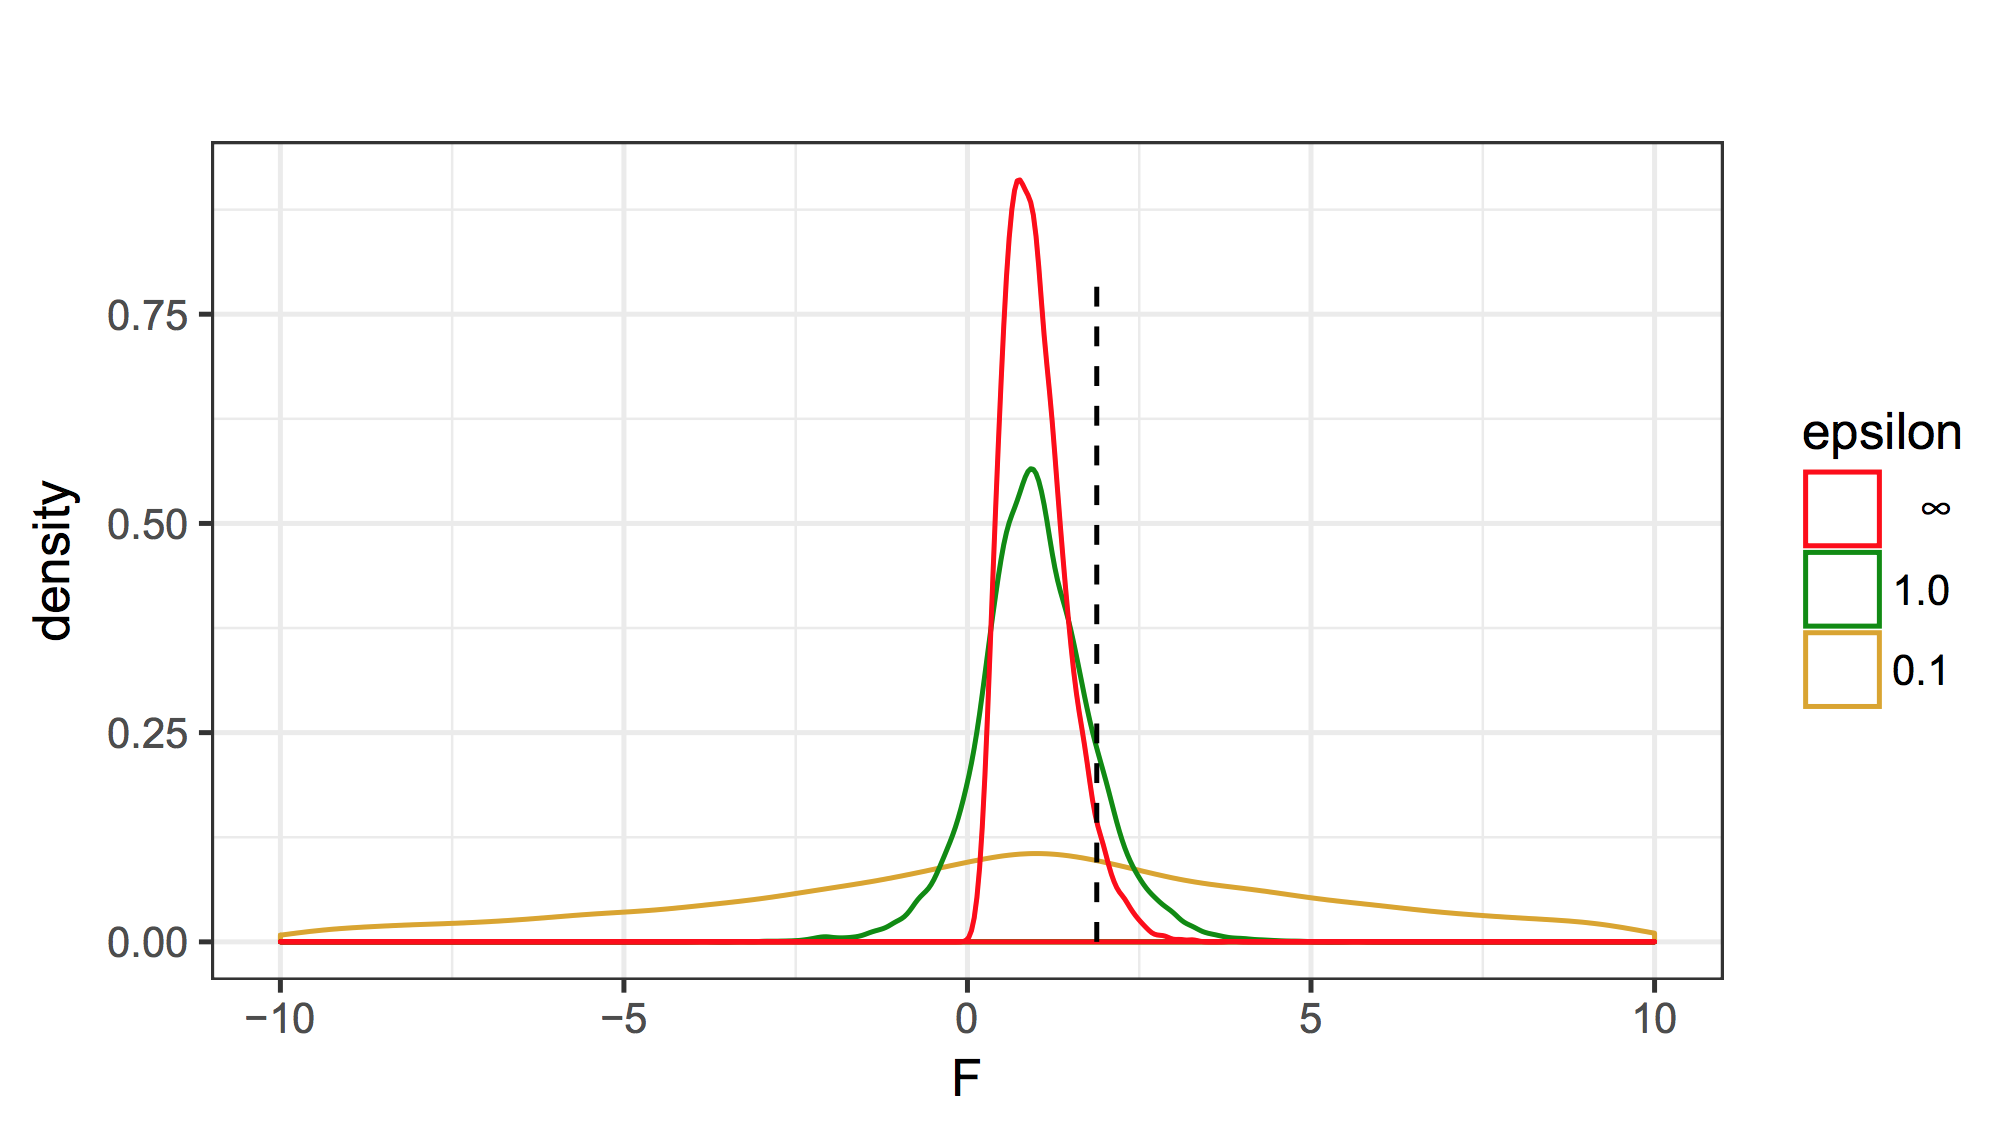
\includegraphics[scale=0.35]{images/noisy-ref-dist}
\end{figure} 
\end{frame}


\begin{frame}{Private ANOVA [CBRG18]}
  \begin{figure}
  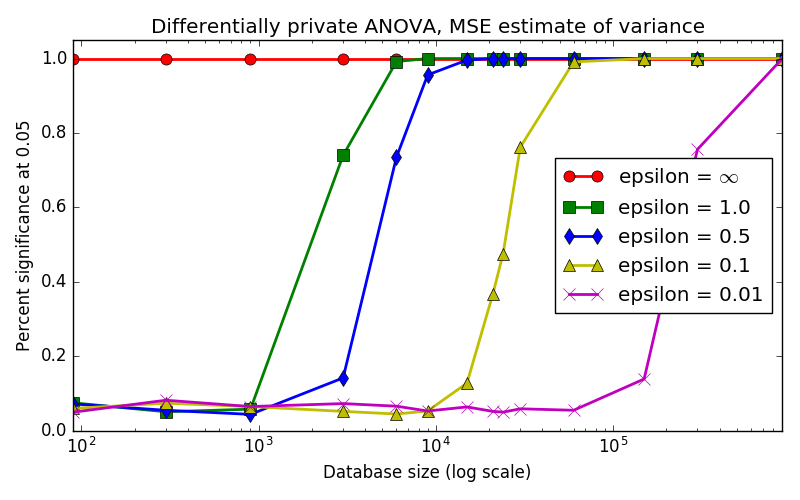
\includegraphics[scale=0.45]{images/campbellpower}
  \end{figure}
  \centering
 Fixed effect size: $\mu = [0.35, 0.5, 0.65], \sigma = 0.15$.
\end{frame}


\begin{frame}{Improving Private ANOVA [\textcolor{blue}{S}HGRGB19]}
\pause
Are there other ways of measuring ``dispersion'' (analogous to variance)? \pause
$$(x_i - \bar{x})^2, \quad \lvert x_i - \bar{x} \rvert, \text{ or maybe }\lvert x_i - \bar{x} \rvert^?$$  \pause
\begin{align*}
\ssa(D) = \sum_{j=1}^{k} n_j (\bar{y}_j - \bar{y})^2  &\Longrightarrow \textcolor{blue}{ \sa(D) = \sum_{j=1}^{k} n_j |\bar{y}_j - \bar{y}| }\\  
\sse(D) = \sum_{i=1}^{n}  (y_{i}-\bar{y}_{c_i})^2  &\Longrightarrow \textcolor{blue}{\se(D) = \sum_{i=1}^{n}  |y_{i}-\bar{y}_{c_i}| } \\  
F(D) = \frac{\ssa(D)/(k-1)}{\sse(D)/(n-k)} &\Longrightarrow  \textcolor{blue} {F_1(D) = \frac{\sa(D)/(k-1)}{\se(D)/(n-k)}}
\end{align*}
 \pause
The new $F_1$ statistic has: \pause
\begin{itemize}
\item Lower sensitivity (3 for \se, 4 for \sa) \pause
\item Much higher typical value 
\end{itemize}
\end{frame}



\begin{frame}{Improving Private ANOVA [\textcolor{blue}{S}HGRGB19]}
Computing $F_1$ privately \pause
\begin{enumerate}
	\item $\widehat{\sa}  = \sa + \lap(4/\rho\varepsilon)$
    \item $\widehat{\se} = \sa + \lap(3/(1-\rho)\varepsilon)$ \pause
    \item $\widehat{F}_1 = \frac{\widehat{\sa}/(k-1)}{\widehat{\se}/(n-k)}$ \pause
\end{enumerate}
Where $\rho$ denotes epsilon allocation
\begin{itemize}
	\item Empirically checked: optimal $\rho \approx 0.7$ \pause
\end{itemize}
Computing accurate $p$-values \pause
\begin{itemize}
	\item Simulate reference distribution of $\widehat{F}_1$ \pause
	\item Problem: reference distribution depends on $\sigma$
\end{itemize}
\end{frame}


\begin{frame}{Improving ANOVA [\textcolor{blue}{S}HGRGB19]}
Need private estimate of $\sigma$ \pause
\begin{itemize}
	\item Allocate some of epsilon budget? \pause
	\item Solution: derive an unbiased estimator for $\sigma$ \pause
\end{itemize}
\bigskip

$$\hat{\sigma} = \sqrt{\pi/2} \cdot \frac{\widehat{SE}}{(N-k)} $$ \pause
\bigskip
Proceed with simulation
\bigskip

Empirically verified to have valid $p$-values.
\end{frame}


\begin{frame}{}
  \begin{figure}
  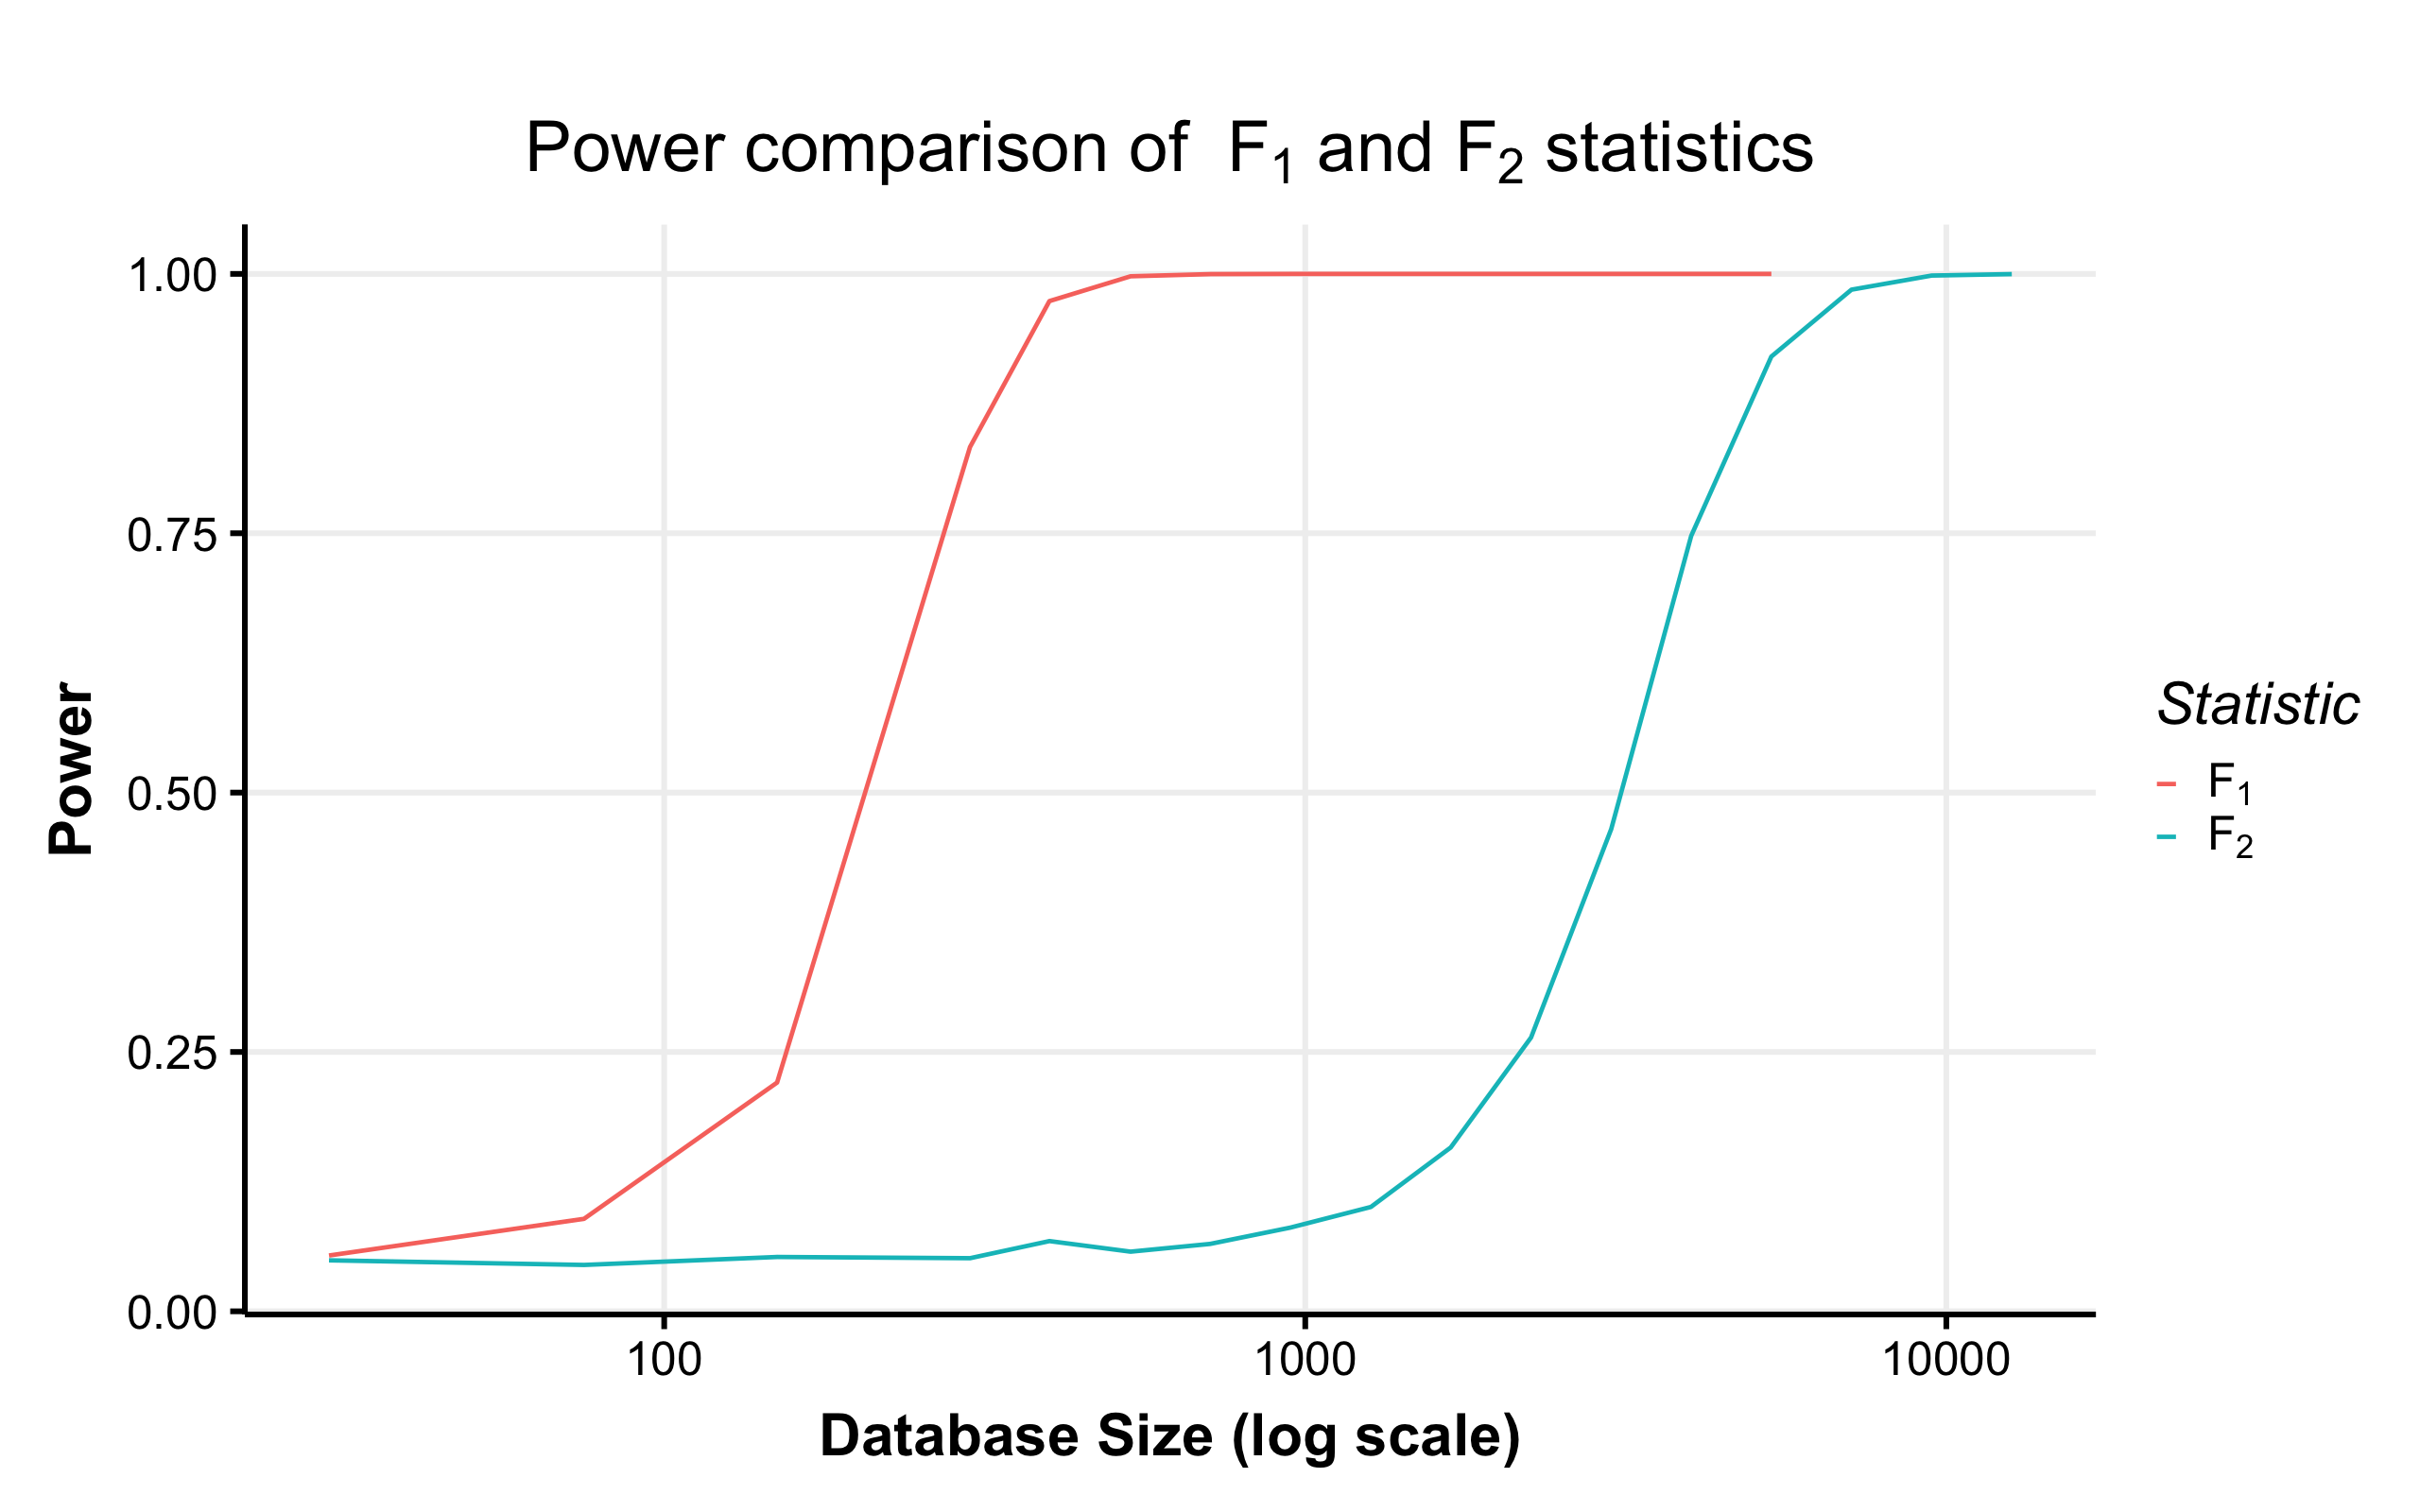
\includegraphics[scale=0.12]{images/f1-vs-f2}
  \end{figure}
  \centering
 \small  Fixed effect size: $\mu = [0.35, 0.5, 0.65], \sigma = 0.15$, and $\varepsilon = 1$.
  
  \pause
  \centering
  \large \textcolor{blue}{Optimal public test $\centernot \implies $ optimal private test}

\end{frame}

\begin{frame}{Further Optimization}
\pause
Are there other ways of measuring ``dispersion'' (analogous to variance)? 
$$(x_i - \bar{x})^2, \quad \lvert x_i - \bar{x} \rvert, \text{ or maybe }\lvert x_i - \bar{x} \rvert^?$$  \pause

Perhaps a different exponent? \pause Turns out 1 is optimal.
\end{frame}

\begin{frame}{Conclusion}
\pause
\large In the private framework \ldots \par \pause
 \normalsize
\begin{itemize}
	\item Not limited to test statistics with closed-form reference distributions \pause
	\item Opportunity for significant power gains \pause
	\item Optimal public test $\centernot \implies$ optimal private test \pause
\end{itemize}

\large \ldots all of statistics is fair game. \pause
 \normalsize
 
 \begin{block}{New developments}
[CKSBG19] gained another order of magnitude improvement. See \textit{Differentially Private Nonparametric Hypothesis Testing} at CCS `19.
 \end{block} \pause
Funding
\begin{figure}
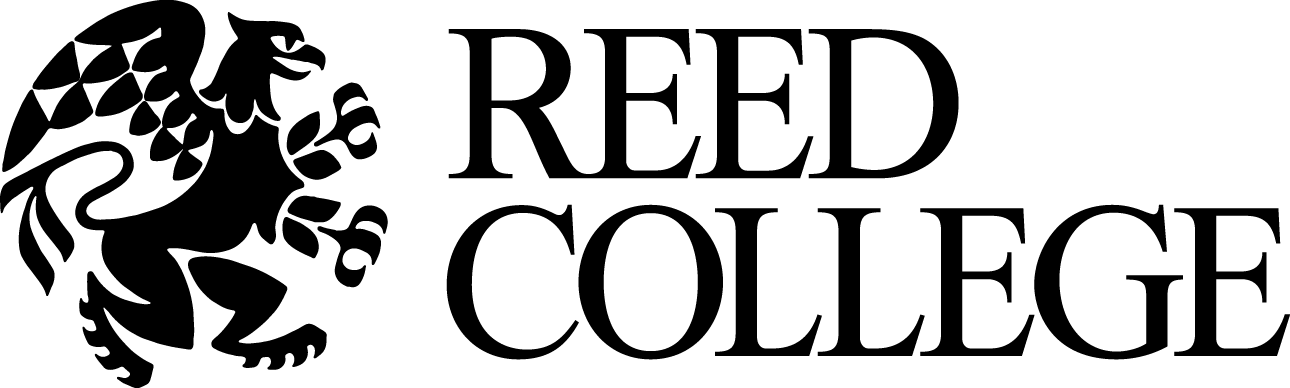
\includegraphics[width=0.4\textwidth]{images/reed-logo}%

\includegraphics[width=0.2\textwidth]{images/NSF-logo}
\end{figure}

%This material is based upon work supported by the National Science Foundation under Grant No. SaTC-1817245 and by the Gillespie Family Student Research Fund.
\end{frame}


\end{document}
